\section{Skill Runtime with JIT Optimization}
\label{sec:runtime}

\begin{figure*}[t]
  \centering
  \setlength{\abovecaptionskip}{3pt}
  \setlength{\belowcaptionskip}{0pt}
  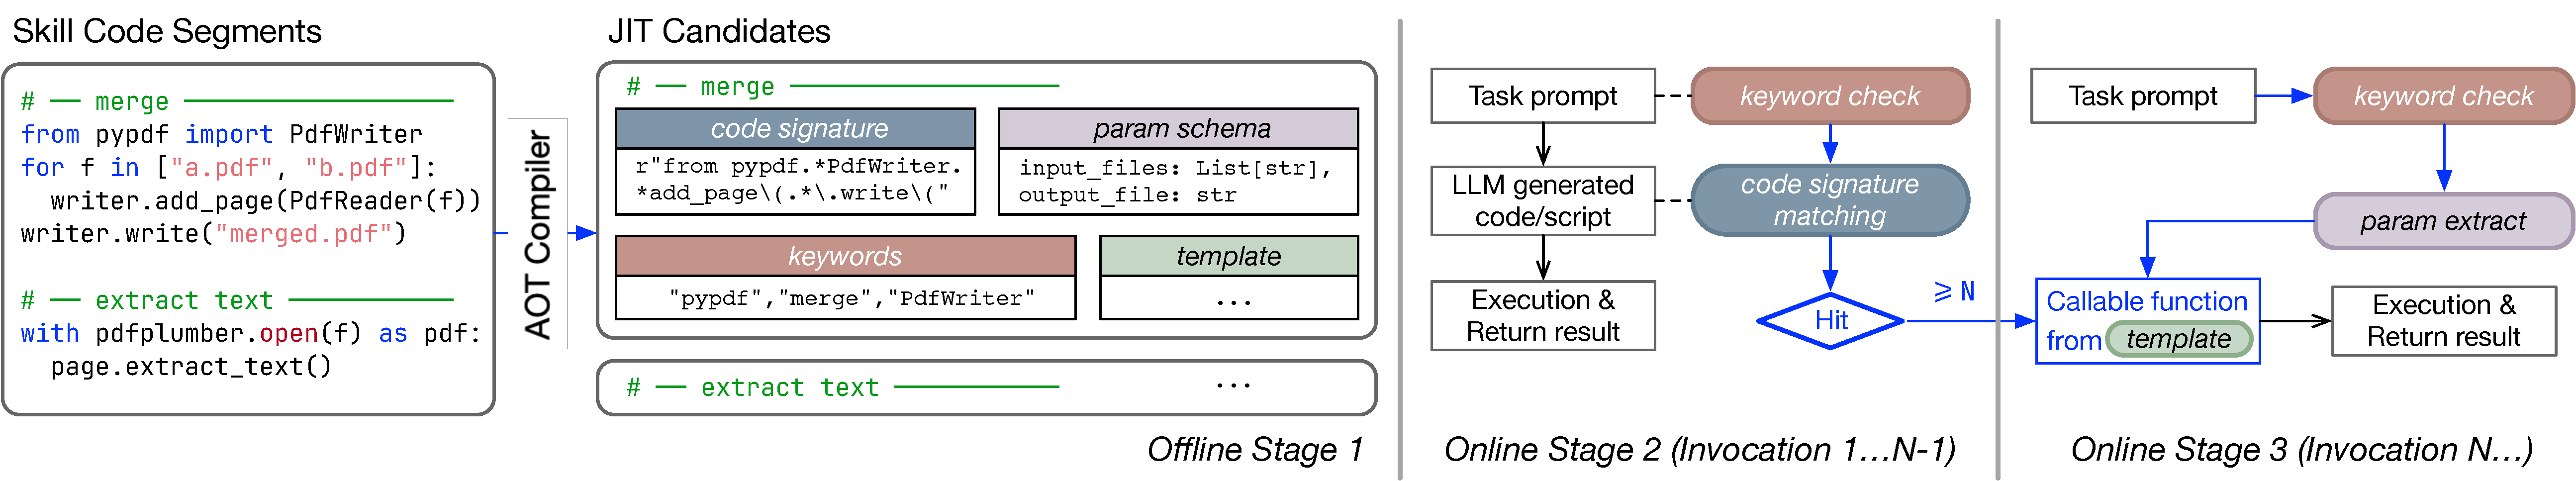
\includegraphics[width=\textwidth]{figures/code_solidification_pipeline.pdf}
  \caption{Code solidification pipeline. The AOT compiler
    analyzes skill code segments and generates JIT candidates
    with code signatures and templates (Stage~1). The runtime
    validates predictions across invocations (Stage~2). After
    promotion, a compiled function replaces LLM inference
    (Stage~3).}
  \label{fig:solidification}
\end{figure*}

AOT compilation generates multiple skill variants for different targets.
Consequently, at runtime, \sys loads the skill variant compiled for the current target.
Since AOT compilation is performed only once per skill and target (model+harness) pair, the compilation overhead is modest.

However, some problems only surface at execution time, such as
capability gaps that static profiling missed or resource
contention among parallel sub-agents competing for
rate-limited APIs. Other opportunities, like code patterns
that recur across invocations, only become visible after
repeated runs. The \sys runtime addresses both through
JIT optimization (\S\ref{sec:runtime:jit}) and a
resource-aware scheduler (\S\ref{sec:runtime:sched}).

\subsection{Skill Registration and Execution}
\label{sec:runtime:exec}

Compilation produces multiple skill variants for each skill,
along with the env-binding scripts generated by Pass~2.
When a new task arrives, the runtime selects the variant
compiled for the current (model, harness) pair.
From the agent's perspective, the complexity of multiple
variants is invisible: it sees a single set of skills and
loads them through the same progressive disclosure mechanism
described in \S\ref{sec:insight}. Before loading the full
skill context, the runtime will first execute the
env-binding script to verify whether runtime dependencies are
satisfied. 

\subsection{JIT Optimization}
\label{sec:runtime:jit}

Beyond AOT compilation, which tailors primitive capabilities
to each target, \sys further applies JIT optimization to
enhance execution quality and efficiency through two
complementary mechanisms: adaptive recompilation and code solidification.

\subsubsection{Adaptive Recompilation}
\label{sec:runtime:jit1}

The runtime tracks the outcome of every task executed with
a skill. When a skill execution fails (e.g., agent abort, human feedback) or retries during the agent loop, the runtime records
a structured failure or retry log. Although the current model may perform self-correction through reflection,
the correction process is not recorded, leading to the possibility of encountering the same errors in subsequent executions.

When the same skill fails across multiple invocations, the
runtime analyzes whether the failures are task-specific or reflect a systematic
capability gap in the skill itself. Only in the latter case
does the runtime trigger adaptive recompilation: it feeds
the accumulated failure logs and the model's self-recovery
traces as input to the compiler, which then applies targeted
compensation transforms to the skill.
If the recompiled variant performs worse, the runtime
rolls back to the previous version. Each subsequent
recompilation starts from the best-performing variant
observed so far, ensuring that optimization is improving skill performance.

\begin{figure*}[t]
  \centering
  \setlength{\abovecaptionskip}{0pt}
  \setlength{\belowcaptionskip}{0pt}
  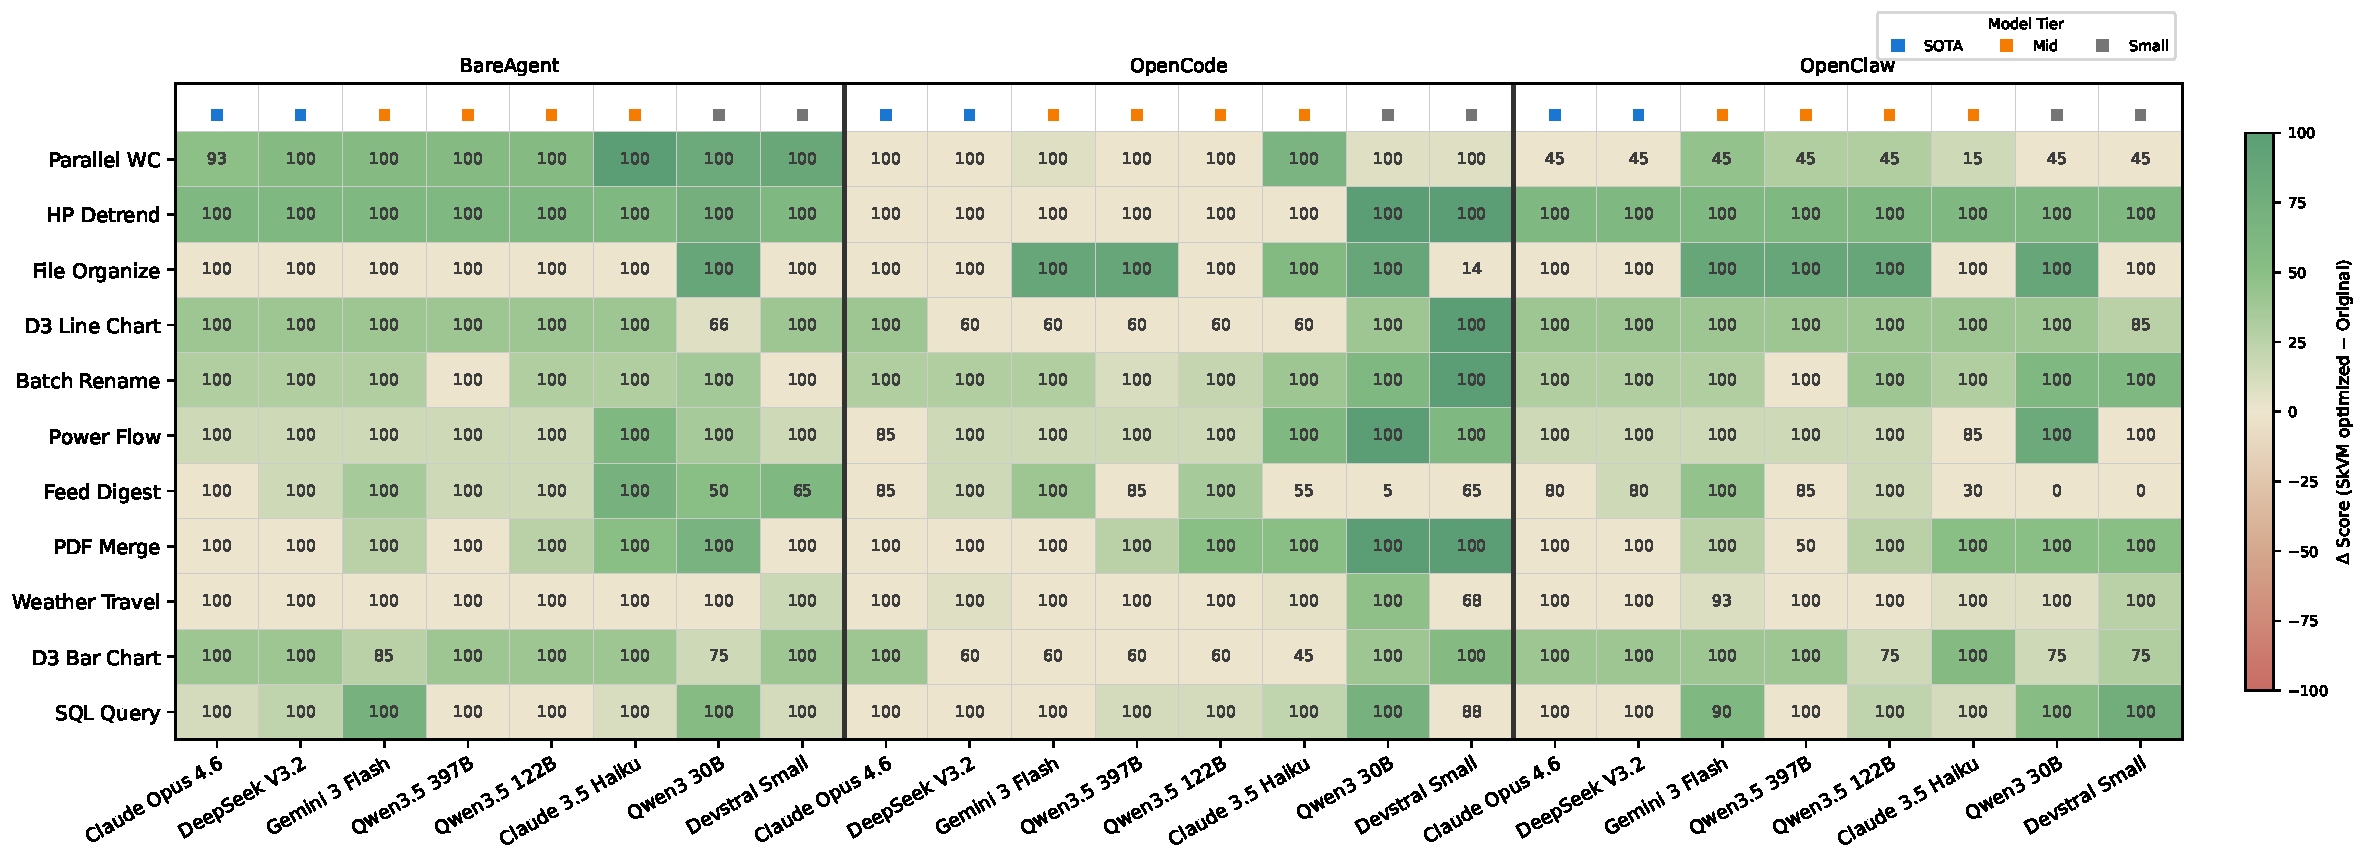
\includegraphics[width=\textwidth]{figures/e1_heatmap.pdf}
  \caption{Skill compilation effectiveness. Cell values represent task completion rates after \sys optimization,
  while cell color indicates the score improvement (green) or regression (red) relative to original baseline skills.}
  \label{fig:e1_heatmap}
\end{figure*}

\subsubsection{Code Solidification}
\label{sec:runtime:jit2}
Recall that 75\% of skills contain solidifiable code
(\S\ref{sec:insight:analysis}): code whose overall structure
is fixed, varying only in input-specific parameters.
In normal execution, the LLM re-executes the full
reasoning and tool-use cycle on every invocation, spending
tokens and latency on a process whose structure is identical
each time. Code solidification identifies these
repetitive patterns and promotes them into executable code
that bypasses model inference.
Figure~\ref{fig:solidification} illustrates the three-stage
pipeline.

In the first stage, the AOT compiler analyzes code and
script segments within each skill, identifying whether
they contain parameterized patterns eligible for
solidification. For eligible segments, it generates a
\emph{JIT candidate} containing four components: keywords
that filter relevant invocations, a \emph{code signature}
that captures the expected output structure as a match
pattern, a code template with parameter slots, and a
parameter schema describing the extractable arguments.
These candidates are bundled with the compiled skill variant.

In the second stage, the runtime monitor watches LLM
invocations across repeated calls. For each invocation,
it first checks keywords for relevance, then matches the
generated code against the code signature. 
The code solidification is triggered only after
the code signature matches successfully across multiple consecutive invocations,
ensuring that the code structure generated by the LLM remains consistent with the patterns analyzed in the AOT stage.
If the model's output consistently
diverges from the code signature, the system stays on
the safe LLM path and never promotes.


In the third stage, the template is instantiated into a callable
function: the template code is wrapped with parameter
extraction and output handling to produce a standalone
shell script or code function. This instantiation step
is lightweight and mechanical, as the AOT stage has already
done the analysis. Subsequent invocations bypass the LLM
entirely: the runtime extracts parameters from the task
context, calls the instantiated function, and returns the
result. If the solidified code execution causes an agent
task to fail or encounters a runtime exception, \sys triggers
a fallback mechanism that re-enables LLM-based code generation
to ensure correctness.

\subsection{Resource-Aware Parallel Scheduling}
\label{sec:runtime:sched}

In Pass~3 of AOT compilation, the compiler identifies where parallelism is
possible, but how much parallelism is \emph{efficient}
depends on conditions that change at run time: CPU usage,
external API rate limit, the machine's available
memory, and other shared resources.

\sys dynamically monitors system state and schedules task execution accordingly,
bridging the gap between compile-time opportunity and run-time reality.
For API-bound workloads, it watches response latencies and HTTP 429 (rate limit) signals.
For compute-bound workloads, it monitors CPU and memory usage.
When pressure rises above a threshold, 
\sys applies two mechanisms to mitigate resource contention.
First, it throttles the launch of new sub-agents to avoid introducing additional concurrency pressure.
Second, for sub-agents that are already running, \sys selectively suspends a subset of them (i.e., pauses their agent-loop execution), based on per-agent resource usage or launch order, to reduce active competition for shared resources.
\sys also records the effective concurrency of each skill from its previous run on the current system and uses it as a concurrency hint for subsequent executions.


